\documentclass[a4paper,10pt,titlepage]{article}
% Språk och encodings
\usepackage[swedish,english]{babel}
\usepackage[T1]{fontenc}
\usepackage[utf8]{inputenc}
\usepackage[fixlanguage]{babelbib}
% Images and floats
\usepackage{graphicx}
\usepackage{wrapfig}
\usepackage{float}
% Clear type + Sans-serif font
\usepackage{lmodern}
\renewcommand{\familydefault}{\sfdefault}
% Avancerade tabeller
\usepackage{tabularx}
\usepackage{multirow}
\usepackage{booktabs}
% Matte
\usepackage{amsmath, amsthm, amssymb}
% Algoritmer
\usepackage[ruled,vlined]{algorithm2e}
% Källkod
\usepackage{listings}
\lstset{
	showspaces = false,
	showstringspaces = false,
}
% Inkludera pdf-sidor
\usepackage{pdfpages}
% Länkar
\usepackage{color}
\definecolor{dark-blue}{rgb}{0, 0, 0.6}
\usepackage{hyperref}
\hypersetup{
  colorlinks=true,
  linkcolor=dark-blue,
  urlcolor=dark-blue
}
% Vettiga paragrafer
\setlength{\parindent}{0pt}
\setlength{\parskip}{2ex}

% Kommando för kommandorader
\newcommand{\cmdline}[1]{\mbox{\textbf{\texttt{> #1}}}}

% Sidhuvud/sidfot
\usepackage{fancyhdr}
\setlength{\headheight}{15pt}
\pagestyle{fancyplain}
\lfoot{Carl-Oscar Erneholm \\ 880422-0872 \\ coer@kth.se}
\rfoot{Martin Nycander \\ 881028-0076 \\ mnyc@kth.se}
\cfoot{Sida \thepage}

% Språk
\selectbiblanguage{swedish}
\selectlanguage{swedish}

% Titel
\title{Laborationsrapport 2 \\ Small-Shell v2.51 för UNIX}
\author{Carl-Oscar Erneholm \and Martin Nycander}
\date{\today}

\begin{document}

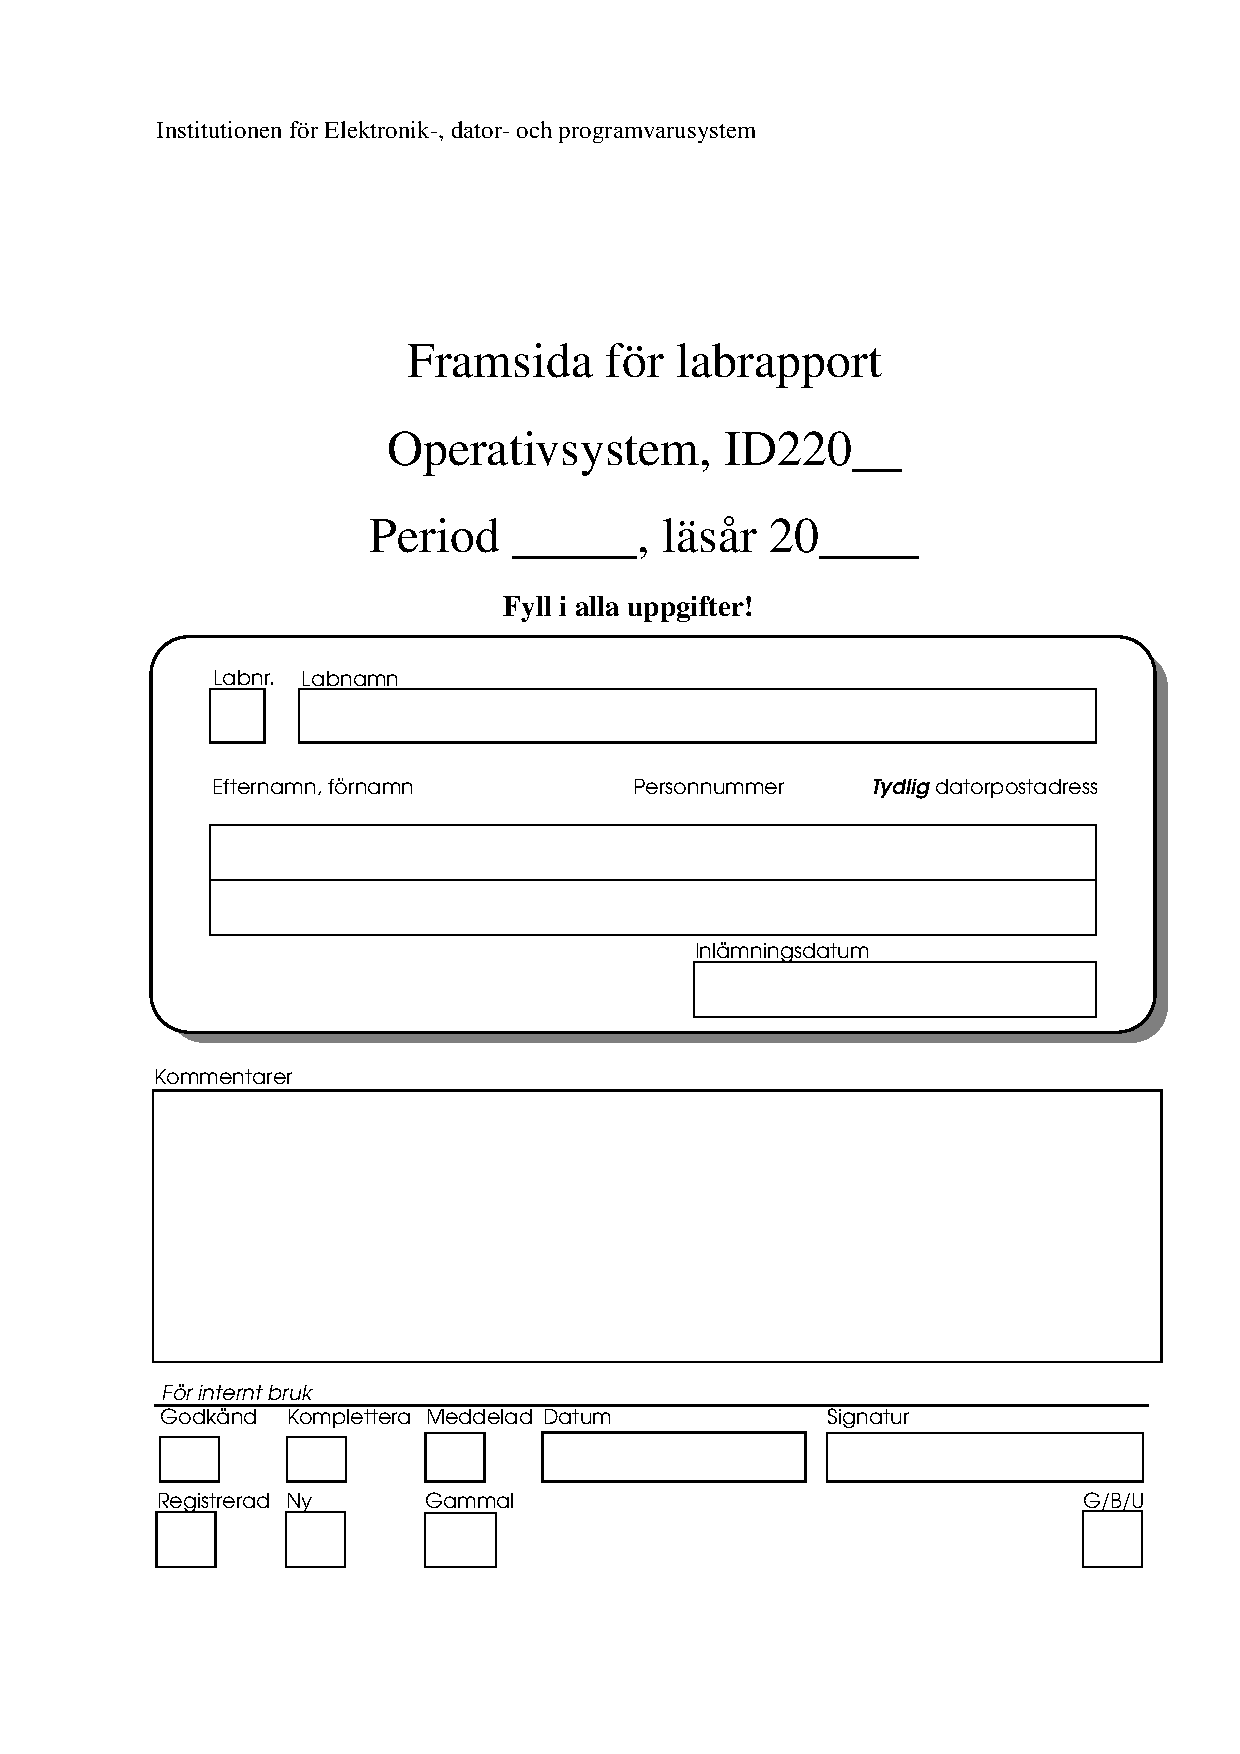
\includepdf[pages=-]{framsida.pdf}

\maketitle

\tableofcontents
\thispagestyle{empty}
\newpage
\setcounter{page}{1}
\section{Problembeskivning}

\subsection{Förberedelsefrågor}


\begin{enumerate}
	\item[1.] \textbf{\footnotesize Motivera varför det ofta är bra att exekvera kommandon i en separat process.}
	
	\verb!//TODO!

	\item[2.] \textbf{\footnotesize Vad händer om man inte i kommandotolken exekverar wait() för en barn-process som avslutas?}
	
	\verb!//TODO!


	\item[3.] \textbf{\footnotesize Hur skall man utläsa SIGSEGV?}
	
	\verb!//TODO!


	\item[4.] \textbf{\footnotesize Varför kan man inte blockera SIGKILL?}
	
	\verb!//TODO!


	\item[5.] \textbf{\footnotesize Hur skall man utläsa deklarationen void (*disp)(int))?}
	
	\verb!//TODO!


	\item[6.] \textbf{\footnotesize Vilket systemanrop använder sigset(3C) troligtvis för att installera en signalhanterare?}
	
	\verb!//TODO!


	\item[7.] \textbf{\footnotesize Hur gör man för att din kommandotolk inte skall termineras då en förgrundsprocess i den termineras med <Ctrl-c>?}
	
	\verb!//TODO!


	\item[8.] \textbf{\footnotesize Studera körningsexemplet nedan och förklara varför man inte har bytt “working directory” till /home/ds/robertr när man avslutat miniShell:et?}
	
	\verb!//TODO!




\end{enumerate}

\newpage
\section{Programbeskrivning}

\newpage
\section{Tester}

För att testa funktionaliten av vårat program har vi valt att köra följande kontrollerade tester:

\begin{table}[H]
	% PAGER satt
	\begin{tabularx}{\textwidth}{>{\bfseries}r  X }
		\multicolumn{2}{c}{\large\textbf{Testfall 1}} \\[0.1cm]
		\toprule	Beskrivning				& Inläsning av PAGER-variabeln \\
		\midrule	Förkrav					& Miljövariabeln \texttt{PAGER} är satt till ``pg''. \\
		\midrule	Körning					& \cmdline{./digenv} \\
		\midrule	Förväntat resultat		& Programmet ``pg'' startas med godtyckligt innehåll. \\
		\bottomrule
	\end{tabularx}
\end{table}

\begin{table}[H]
	% PAGER inte satt (med less)
	\begin{tabularx}{\textwidth}{>{\bfseries}r  X }
		\multicolumn{2}{c}{\large\textbf{Testfall 2}} \\[0.1cm]
		\toprule	Beskrivning				& Misslyckad inläsning av PAGER-variabeln \\
		\midrule	Förkrav					& Miljövariabeln \texttt{PAGER} finns inte, programmet ``less'' finns i path:en. \\
		\midrule	Körning					& \cmdline{./digenv} \\
		\midrule	Förväntat resultat		& Programmet ``less'' startas med godtyckligt innehåll. \\
		\bottomrule
	\end{tabularx}
\end{table}

\begin{table}[H]
	% PAGER inte satt (utan less)
	\begin{tabularx}{\textwidth}{>{\bfseries}r  X }
		\multicolumn{2}{c}{\large\textbf{Testfall 3}} \\[0.1cm]
		\toprule	Beskrivning				& Misslyckad inläsning av PAGER-variabeln, utan ``less'' \\
		\midrule	Förkrav					& Miljövariabeln \texttt{PAGER} finns inte, programmet ``less'' finns inte i path:en. Programmet ``more'' finns i path:en. \\
		\midrule	Körning					& \cmdline{./digenv} \\
		\midrule	Förväntat resultat		& Programmet ``more'' startas med godtyckligt innehåll. \\
		\bottomrule
	\end{tabularx}
\end{table}

\begin{table}[H]
	\begin{tabularx}{\textwidth}{>{\bfseries}r  X }
		\multicolumn{2}{c}{\large\textbf{Testfall 4}} \\[0.1cm]
		\toprule	Beskrivning				& Normal användning med filtrering \\
		\midrule	Förkrav					& Miljövariabeln \texttt{PAGER} är satt till ``less''. \\
		\midrule	Körning					& \cmdline{./digenv PATH} \\
		\midrule	Förväntat resultat		& \begin{itemize}
  			\setlength{\itemsep}{0pt}
  			\setlength{\parskip}{0pt}
  			\setlength{\parsep}{0pt}
			\item Utskrift och tillstånd ska vara ekvivalent med: \cmdline{printenv | grep PATH | sort | less}
			\item Inga oavslutade barn-procceser finns. Verifiera med \cmdline{ps -ef}.
			\item Inga temporära datafiler har skapats.
		\end{itemize} \\
		\bottomrule
	\end{tabularx}
\end{table}

\begin{table}[H]
	\begin{tabularx}{\textwidth}{>{\bfseries}r  X }
		\multicolumn{2}{c}{\large\textbf{Testfall 5}} \\[0.1cm]
		\toprule	Beskrivning				& Normal användning med filtrering och flaggor \\
		\midrule	Förkrav					& Miljövariabeln \texttt{PAGER} är satt till ``less''. \\
		\midrule	Körning					& \cmdline{./digenv -i pAtH} \\
		\midrule	Förväntat resultat		& Samma som testfall 3. \\
		\bottomrule
	\end{tabularx}
\end{table}

\begin{table}[H]
	\begin{tabularx}{\textwidth}{>{\bfseries}r  X }
		\multicolumn{2}{c}{\large\textbf{Testfall 6}} \\[0.1cm]
		\toprule	Beskrivning				& Syntaxfel i argument till grep \\
		\midrule	Förkrav					& - \\
		\midrule	Körning					& \cmdline{./digenv -.} \\
		\midrule	Förväntat resultat		& \begin{itemize}
  			\setlength{\itemsep}{0pt}
  			\setlength{\parskip}{0pt}
  			\setlength{\parsep}{0pt}
			\item Programmet avbryts.
			\item Ett felmeddelande kan skrivas till \texttt{stderr}.
			\item Resultatet av ``\cmdline{echo \$?}'' ska inte bli $0$.
			\item Inga oavslutade barn-procceser finns. Verifiera med \cmdline{ps -ef}.
			\item Inga temporära datafiler har skapats.
		\end{itemize} \\
		\bottomrule
	\end{tabularx}
\end{table}

\newpage
\section{Resultat}

Körning av ovanstående standardiserade testfall gav följande resultat.

\begin{tabularx}{\textwidth}{>{\bfseries}l  X }
	\multicolumn{2}{c}{\large\textbf{Testfallsresultat}} \\[0.1cm]
	\toprule
	1. ??? 							& ??? \\
	\bottomrule
\end{tabularx}


\newpage
\section{Labbutvärdering}


\newpage
\section{Källkod}

\lstset{tabsize=2}
\footnotesize{\lstinputlisting[language=C]{../program/minishell.c}}


\end{document}